
\title{Лекция 1\\Основные положения семантической технологии проектирования интеллектуальных компьютерных систем нового поколения \vspace{-2em}} 
\author[]{Шункевич Д.В.}
\institute[]{Белорусский государственный университет информатики и радиоэлектроники}

\begin{frame}
	\titlepage
\end{frame}

\begin{frame}{\\Содержание лекции}
	\vspace{10mm}
	\topline
	\justifying
		Интеллектуальная система, комплексная задача, гибридная интеллектуальная система.
		Основные положения семантической технологии проектирования интеллектуальных компьютерных систем нового поколения.
		Основные компоненты указанной технологии.
		Информационная конструкция, формальный язык, знак, синтаксис, семантика.
		Семантическая память.
\end{frame}

\begin{frame}{\\Интеллектуальная система}
	\topline
	\justifying
	\begin{SCn}
		\scnheader{интеллектуальная система} 
		\scnidtf{система, которая может легко \underline{научиться решать} новые задачи} 
		\begin{scnrelfromset}{важно отличать}
			\scnitem {способность обучаться более \underline{качественному решению} задач \underline{одного ограниченного} класса (как это делают нейросетевые модели)}
			\scnitem {способность обучаться решению задач \underline{разных} классов (с ограничениями или без них)}
		\end{scnrelfromset}
	\end{SCn}
\end{frame}

\begin{frame}{\\Комплексная задача}
	\topline
	\justifying
	\begin{SCn}
		\scnheader{комплексная задача}
		\scnidtf{задача, для решения которой необходимо использовать различные виды знаний и различные модели решения задач}
			\begin{scnrelfrom}{примечание}
	 			{Для решения комплексных задач невозможно заранее определить набор моделей решения задач}
			\end{scnrelfrom}
		\vspace{5mm}
		\textbf{Примеры комплексных задач:}
		\begin{textitemize}
			\item{задача понимания естественных языков, изображений, речевых сообщений}
			\item{задача планирования поведения интеллектуальных роботов}
		\end{textitemize}
	\end{SCn}
\end{frame}

\begin{frame}{\\Гибридная интеллектуальная система}
	\topline
	\justifying
	\vspace{10mm}
	\begin{SCn}
		\scnheader{гибридная интеллектуальная система} 
		\scnidtf{интеллектуальная система, интегрирующая различные виды знаний и различные модели решения задач}
		\begin{scnrelfrom}{примечание}
			{ГИС ориентированны на решение комплексных задач}
		\end{scnrelfrom}
		\begin{scnrelfromset}{недостатки современного состояния}
				\scnitem{монолитность}
				\scnitem{ориентированность на решение задачи одного класса (не нескольких различных классов задач)}
				\scnitem{требование колоссальных ресурсов (времени) для разработки систем}
				\scnitem{невозможность повторного использования компонентов систем для решения других задач (как следствие монолитности)}
		\end{scnrelfromset}
	\end{SCn}
\end{frame}

\begin{frame}{\\Технология OSTIS}
	\topline
	\justifying
	\vspace{10mm}
	\begin{SCn}
		\scnheader{OSTIS}
		\scnidtf{Open Semantic Technology for Intelligent Systems}
		\scnidtf{открытая комплексная технология проектирования совместимых интеллектуальных систем}
	
		\begin{scnrelfromset}{основные положения}
			\scnitem {база знаний OSTIS может описывать \underline{любой вид} знаний}
			\scnitem {решатель задач OSTIS основан на многоагентном подходе и позволяет легко \underline{комбинировать любые модели} решения задач}
			\scnitem {интерфейс ostis-системы представляет собой подсистему со своей БЗ и решателем задач (также может быть описан с помощью SC-кода)}
			\scnitem {использование \underline{универсального} способа представления (кодирования) информации, получившего название SC-код}
		\end{scnrelfromset}
	\end{SCn}
\end{frame}

\begin{frame}{\\}	
	\topline
	\justifying
	\vspace{10mm}
	\begin{SCn}
	\scnheader{OSTIS}
	\begin{scnrelfromset}{достоинства}
		\scnitem {унифицированность представления (любая информация представляется \underline{одинаково})}
		\scnitem {удобство машинной обработки и восприятия человеком}
		\scnitem {любые знания и модели решения задач легко интегрируются в ostis-систему (по принципу plug \& play) и её всегда можно переобучить}
		\scnitem {универсальность и совместимость компонентов (повторное использование позволяет сократить время разработки новых компонентов на 40-60\%)}
		\scnitem {система описывается с помощью SC-кода, поэтому она может \underline{анализировать себя}, искать в себе ошибки и оптимизировать собственную работу (рефлексивность)}
		\end{scnrelfromset}
	\end{SCn}
\end{frame}

\begin{frame}{\\}
	\topline
	\justifying
	\vspace{10mm}
	\begin{SCn}	
		\scnheader{OSTIS}
		\begin{scnrelfromset}{достоинства}
			\scnitem {платформенная независимость (разработка независима от архитектуры компьютера, платформа может быть реализована в программном варианте или в аппаратном)}
			\scnitem {параллельная обработка информации}
			\scnitem {ostis-система может включать в себя компоненты, разработанные на базе OSTIS, и объединяться с другими системами и интегрировать другие компоненты (с помощью JSON или API)}
			\scnitem {производительность ostis-системы не хуже традиционной, а иногда может оказаться лучше за счёт параллельной обработки (при переходе на семантические компьютеры производительность будет ещё выше)}
		\end{scnrelfromset}
	\end{SCn}
\end{frame}
  
\begin{frame}{\\}
	\topline
	\justifying
	\vspace{10mm}
	\begin{SCn}	
		\textbf{Важно понимать:}
			\begin{textitemize}
			\item  {OSTIS -- это не конкретная интеллектуальная система, а \textbf{технология разработки} интеллектуальных систем, каждая из которых будет решать задачи определённого класса}
			\item {ключевые преимущества OSTIS заключаются не в новых функциональных возможностях разрабатываемых систем (большинство функций ostis-систем можно реализовать с помощью традиционных средств), а в том, насколько легко \textbf{модифицировать и развивать} разрабатываемые системы, адаптировать их к новым задачам, а также насколько эффективно можно накапливать и использовать полученные компоненты при разработке новых систем, сокращая при этом время и трудоёмкость их разработки}
			\item {OSTIS -- это способ решения проблемы \textbf{совместимости}, одной из важнейших проблем современных технологий}
			\end{textitemize}
	\end{SCn}
\end{frame}	

\begin{frame}{\\Архитектура ostis-системы}
	\topline
	\justifying
	\vspace{10mm}
	\begin{figure}[H]
		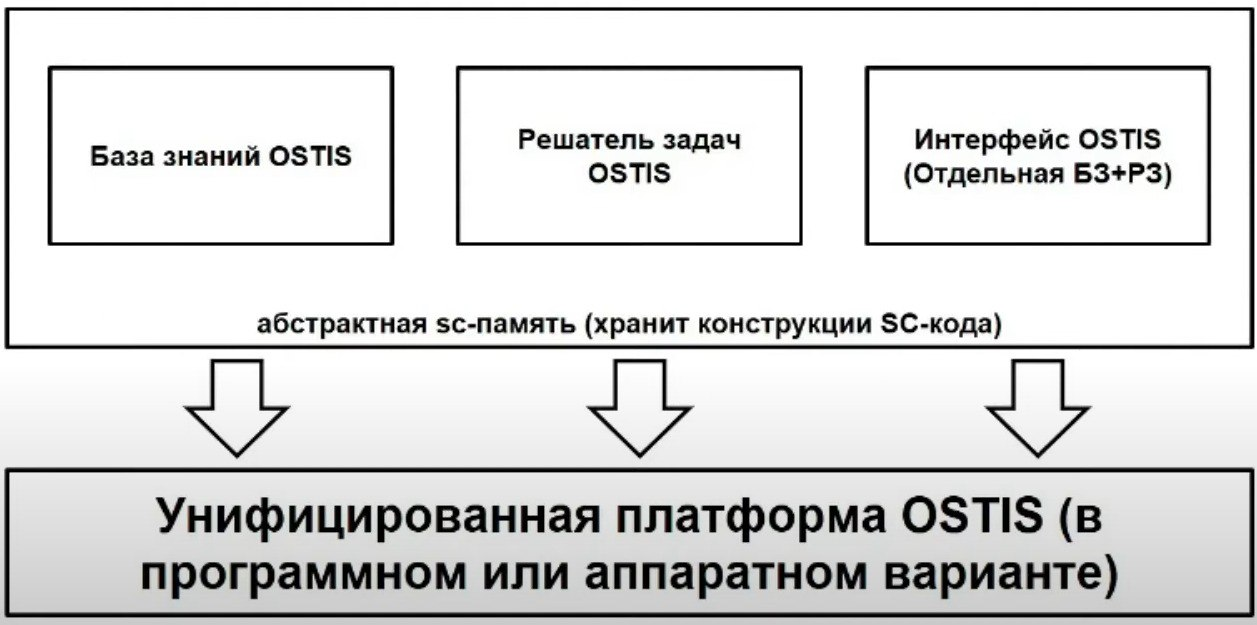
\includegraphics[scale=0.2]{./figures/sd_ostis_basics/scheme.jpeg}
	\end{figure}
\end{frame}

\begin{frame}{\\}
	\topline
	\justifying
	\begin{SCn}	
		\scnheader{база знаний OSTIS}
		\scnidtf{база знаний, описывающая любой вид знаний, при этом её легко дополнять новыми видами знаний}
		\scnheader{решатель задач OSTIS}
		\scnidtf{решатель задач, основанный на многоагентном подходе и позволяющий легко интегрировать и комбинировать любые модели решения задач}
		\scnheader{интерфейс OSTIS}
		\scnidtf{подсистема со своей базой знаний и решателем задач }
		\scnrelfrom{уточнение}{интерфейс так же может быть описан с помощью SC-кода}
	\end{SCn}
\end{frame}

\begin{frame}{\\Информационная конструкция}
	\topline
	\justifying
	\begin{SCn}
		\scnheader{информационная конструкция}
		\scnidtf{конструкция (структура), содержащая некоторые сведения о некоторых сущностях}	
		\scnidtf{информация}
		\scnrelfrom{примечание}{Информационная конструкция имеет форму представления (текст, звук, изображение), форму структуризации (синтаксис), смысл (денотационную семантику)}
	\end{SCn}
\end{frame}

\begin{frame}{\\}
	\topline
	\justifying
		\begin{SCn}
		\scnheader{информационная конструкция}
		\begin{scnrelfromset}{разбиение}
			\scnitem{sc-множество}
				\begin{scnindent}
				\scnidtf{внутренняя информационная конструкция ostis-системы, хранимая в её (внутренней) sc-памяти}
				\end{scnindent}
			\scnitem{файл}
				\begin{scnindent}
				\scnidtf{внутреняя информационная конструкция ostis-системы, хранимая в её файловой (внешней) памяти}
				\scnrelfrom{примечание}{файл может храниться в памяти другой системы}
				\end{scnindent}
			\scnitem{внешняя информационная конструкция, не являющаяся ни файлом, ни sc-конструкцией}
		\end{scnrelfromset}
	\end{SCn}
\end{frame}

\begin{frame}{\\Формальный язык}
	\topline
	\justifying
	\begin{SCn}
		\scnheader{язык}  
		\scnidtf{множество информационных конструкций, построенных по общим синтаксическим и семантическим правилам}
		\begin{scnrelfromset}{разбиение}
			\scnitem{искуственный (построенный) язык}
			\scnitem{формальный язык}
			\scnitem{естественный язык}
		\end{scnrelfromset}
		\scnheader{формальный язык}  
		\scnidtf{язык, в котором значение каждого слова или знака, правила построения предложений и понимания их смысла однозначны}
		\scnidtf{множество строк над конечным алфавитом языка}		
	\end{SCn}
\end{frame}

\begin{frame}{\\Знак}
	\topline
	\justifying
	\begin{SCn}
		\scnheader{знак}
		\scnidtf{фрагмент информационной конструкции, обладающий свойством, \underline{обозначать} некоторую сущность (объект), которая наряду с другими сущностями описывается указанной информационной конструкцией}
		\scnheader{семиотика}
		\scnidtf{наука о знаках}
		\begin{scnrelfromset}{разбиение}
			\scnitem{синтаксис (изучает правильное построение текста)}
			\scnitem{семантика (изучает значение знаков)}
			\scnitem{прагматика (изучает отношение между знаком и субъектом)}
		\end{scnrelfromset}
	\end{SCn}
\end{frame}

\begin{frame}{\\Семантика}
	\topline
	\justifying
	\vspace{10mm}
	\begin{SCn}
		\scnheader{семантическая сеть}
		\scnidtf{граф, вершины которого являются знаками некоторых сущностей, а дуги (ребра) – знаками связей между этими сущностями}
		\scnheader{семантика знака}
		\scnidtf{отношение между знаком и сущностью (значением знака, денотатом), которую он обозначает}
		\begin{figure}[H]
			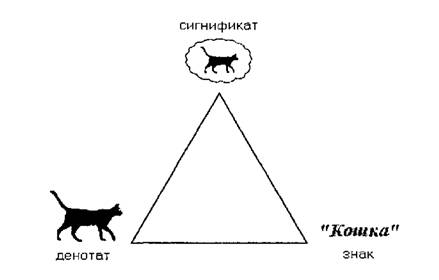
\includegraphics[scale=0.5]{./figures/sd_ostis_basics/sc-code-cat.jpg}
		\end{figure}
	\end{SCn}
\end{frame}

\begin{frame}{\\}
	\topline
	\justifying
	\vspace{15mm}
	\begin{figure}[H]
		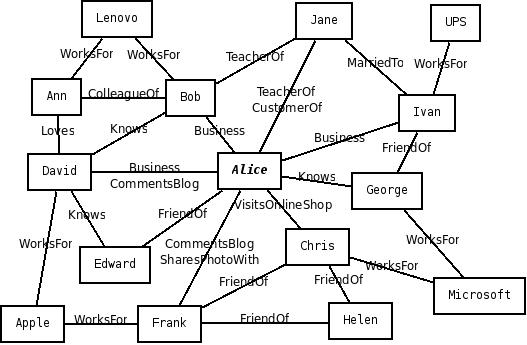
\includegraphics[scale=0.6]{./figures/sd_ostis_basics/sc-code-web.jpg}
		\caption{Пример семантической сети}
	\end{figure}
\end{frame}

\begin{frame}{\\Синтаксис и семантика}
	\topline
	\justifying
	\scnheader{синтаксис}
	\scnidtf{наука, изучающая отношения между знаками}
	\scnrelfrom{примечание}{Синтаксис переводится как порядок, координация}
	\scnheader{семантика}
	\scnidtf{наука, изучающая отношения между знаками и их значениями}
	\scnrelfrom{примечание}{Семантика переводится как обозначение, значение}
\end{frame}

\begin{frame}{\\Семантическая память}
	\topline
	\justifying
	\begin{SCn}
		\scnheader{семантическая память}
		\scnidtf{графодинамическая (нелинейная) память}
		\scnidtf{смысловая память, обеспечивающая хранение семантических сетей}
		\scnrelfrom{примечание}{Изменение семантической памяти происходит не только путем изменения состояния элементов памяти (вершин графа), но также и изменением конфигурации связей между элементами (ребер или дуг графа)}
	\end{SCn}
\end{frame}


